\begin{figure}
    \begin{enumerate}
        \item[(a)] 
\includegraphics[scale=1.05]{plot_rank_similarity_papertop.pdf}\\
        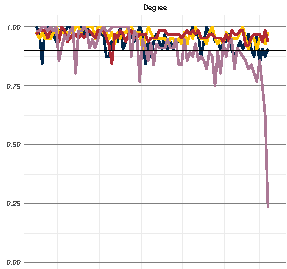
\includegraphics[scale=1.05]{plot_rank_similarity_paper_degree.pdf}\hspace*{0.1mm}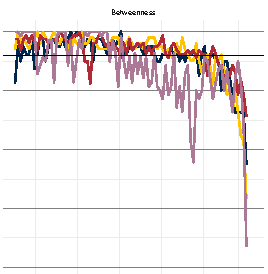
\includegraphics[scale=1.05]{plot_rank_similarity_paper_betweenness.pdf}\hspace*{-0.4mm}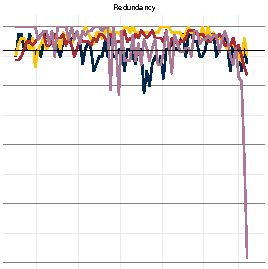
\includegraphics[scale=1.05]{plot_rank_similarity_paper_redundancy.pdf}\\
        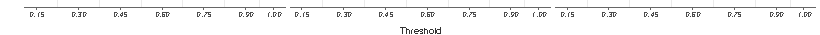
\includegraphics[scale=1.05]{plot_rank_similarity_paperbottom.pdf}
        \vspace*{-0.6cm}
        \item[(b)] \hspace*{-0.25cm}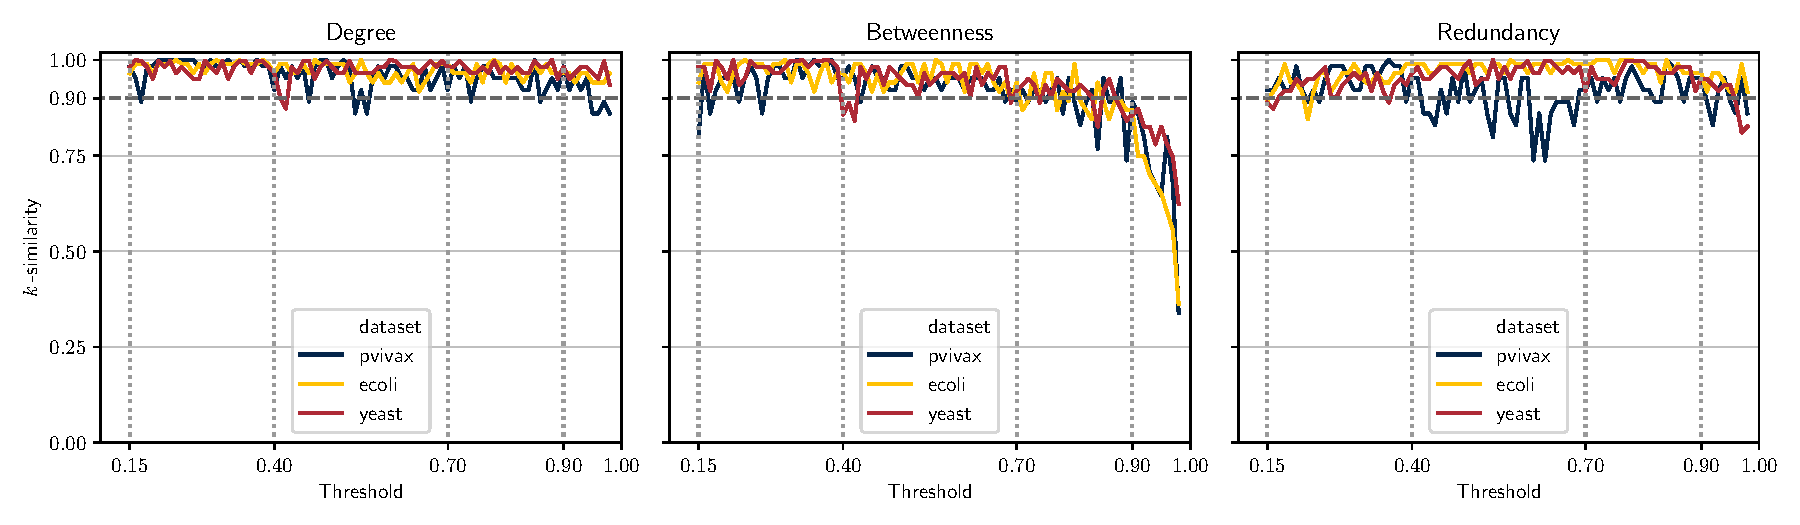
\includegraphics[align=t,width=\linewidth]{plot_rank_similarity_graffs.pdf}
    \end{enumerate}
    \vspace*{-0.6cm}

    \caption{Comparison of $k$-similarity plots from The Paper~(a) and from values calculated by \graffs~(b).
        Each plot shows $k$-similarity between ranks of graphs derived from protein networks at consecutive thresholds.
    The three chosen metrics \texttt{Degree}, \texttt{Betweenness}, \texttt{Redundancy} demonstrate that values obtained by \graffs closely match those from The Paper.}
    \label{fig:plot_rank_similarity}
\end{figure}
